\item A sleeve \( A \) can slide freely along a smooth rod bent in the shape of a half-circle of radius \( R \) (Fig. 1.28). The system is set in rotation with a constant angular velocity \( \omega \) about a vertical axis \( OO' \). Find the angle \( \theta \) corresponding to the steady position of the sleeve.
    \begin{center}
        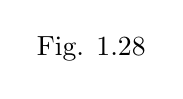
\begin{tikzpicture}
            \node at (0, 0) {Fig. 1.28};
        \end{tikzpicture}
    \end{center}\begin{solution}
    \begin{center}
        \begin{tikzpicture}
            \pic at (0, 0) {frame=3cm};
        \end{tikzpicture}
    \end{center}
    
    \begin{align*}
        \intertext{Let us observe the behaviour of the sleeve in the frame fixed to the rotating rod bent into the shape of half circle. We resolve all the forces into tangential and normal components, then the net downward tangential force on the sleeve is}
        mg \sin \theta \left( 1 - \dfrac{\omega^2 R}{g} \cos \theta \right)
        \intertext{This vanishes for $\theta = 0$ and for $\theta = \theta_0 = \cos^{-1}(g/\omega^2 R)$, which is real if $\omega^2 R > g$.}
        \intertext{If $\omega^2 R < g$, then $[1-(\omega^2 R/g) \cos \theta]$ is always positive for small values of $\theta$ and hence the net tangential force near $\theta=0$ opposes any displacement away from it, and $\theta=0$ is then stable.}
        \intertext{If $\omega^2 R > g$, then $[1-(\omega^2 R/g) \cos \theta]$ is negative for small $\theta$ near $\theta=0$, and $\theta=0$ is then unstable.}
        \intertext{However $\theta = \theta_0$ is stable because the force tends to bring the sleeve near the equilibrium position $\theta = \theta_0$.}
        \intertext{If $\omega^2 R = g$, the two positions coincide and becomes a stable equilibrium point.}
    \end{align*}
\end{solution}